
\chapter{Johdanto}


Järjestelmäintegraatiot \textit{(Enterprise Application Integration, EAI)} tarkoittaa ohjelmistoja, 
jotka yhdistävät eli integroivat organisaation olemassa olevia erillisiä järjestelmiä toimimaan yhdessä.

Tarve EAI:lle kehittyi kun organisaation jo olemassa olevien
järjestelmien hajautunut tieto piti yhdistää tiedonkulun optimoimiseksi ja
automatisoimiseksi. Esimerkiksi organisaation asiakkuudenhallinnasta vastaavan ohjelmiston
pitäisi pystyä keskustelemaan myynninhallinnointiohjelmiston kanssa pitääkseen
asiakastilastot ajan tasalla. 
Järjestelmät jäivät helposti erillisiksi saarekkeiksi eivätkä jakaneet tietoa keskenään. 
Syntyi niin sanottuja "savupiippujärjestelmiä", joissa järjestelmä oltiin suunniteltu pitämään data esimerkiksi firman yksittäisen osaston sisällä, eikä järjestelmän suunnitteluvaiheessa oltu huomioitu datan jakamista; järjestelmästä puuttui esimerkiksi ulospäin suuntavat ohjelmointirajapinnat. 

Järjestelmäintegraatio mahdollistaa näiden eri järjestelmien keskinäisen keskustelun toisilleen. Näin voidaan rakentaa yhteinen järjestelmä jo olemassa olevista palasista \citep[sivu 15]{linthicum2000enterprise}. Useissa tapauksissa organisaation sisäisiä järjestelmiä yhdistetään myös ulkoisiin järjestelmiin tai muiden organisaatioiden kanssa \citep{Johannesson2001}.
Organisaation olemassa olevat järjestelmät voi olla kehitetty eri käyttöjärjestelmille, hyödyntävät eri
ohjelmointikieliä tai tietokantaratkaisuita. Väliin tarvitaan integraatio, joka hoitaa
kommunikoinnin ohjelmistojen välillä


Vuonna 2020 EAI-markkinan arvioitiin olevan 9,26 miljardin dollarin (USD) arvoinen \citep{mordorintelligence} ja koostuu ohjelmistojättien (Microsoft, Oracle, Salesforce IBM) ja pienempien yksittäisten yritysten (Workato, SnapLogic, Tibico) tarjoamista järjestelmistä.

Monet tämän päivän järjestelmäintegraatioalustat tarjoavat joukon työkaluja ja lähestymistapoja, joilla on paljon yhteisiä piirteitä keskenään. Tämän tutkielman tarkoituksena on avata, mistä nämä toisiaan muistuttavat lähestymistavat ovat peräisin, miten niihin on päädytty ja mikä on niiden asema tänä päivänä.

Luku \ref{chap:lähestymis_tavat} kuvaa, miten järjestelmäintegraatioita on lähestytty historiallisesti ja esittelee järjestelmäintegraatioiden merkittävintä kirjallisuutta.

Luku \ref{chap:sanomapohjaiset} paneutuu sanomapohjaisiin suunnittelumalleihin ja erityisesti järjestelmäintegraatioiden suunnittelumalleina \textit{(enterprise integration patterns, EIP)} tunnettuihin lähestymistapoihin ja perehtyy niiden yläkategorioihin ja selittää itse mallien lähestymistapoja ja niiden perusteita. Suunnittelumallien nykytilannetta käsitellään lyhyesti.

Luku \ref{chap:kehitystä} käsittelee, miten järjestelmäintegraatioiden suunnittelumallit ovat asentuneet moderneja teknologioita käyttäviin järjestelmiin ja perehtyy suunnittelumallien heikkouksina pidettyjen piirteiden kehitykseen integraatioalustaympäristössä.


\chapter{Järjestelmäintegraatioiden lähestymistavat} \label{chap:lähestymis_tavat}

Tässä luvussa esitellään suosituimpia jäsentely ja lähestymistapoja järjestelmäintegraatioille. Eri lähestymistavat perustuvat viitatuimpaan järjestelmäintegraatioarkkitehtuurin kirjallisuuteen. Luvun tarkoituksena on antaa kattokategorioita erilaisille teknisille lähestymistavoille ja antaa historiallista kontekstia eri arkkitehtuurisuuntauksille.

\section{Integraatiotasot}

Integraatioiden lähestymistavat voidaan luokitella neljään eri tasoon \citep[sivu 21-23]{linthicum2000enterprise}

\begin{enumerate}
   \item Datatasolla dataa siirretään eri tietovarastojen välillä ja mahdollinen datan prosessointi ja muokkaus toteutetaan siirron yhteydessä. Kyseisellä menetelmällä on myös paljon yhtäläisyyksiä tyypillisen datavaraston \textit{(data warehouse)} toteutuksen kanssa.
   \item Rajapintatasolla pyritään hyödyntämään tarkoitusta varten tilattujen tai paketoitujen sovellusten, esimerkiksi SAP, PeopleSoft, tarjoamia ohjelmointirajapintoja.
   \item Metoditasolla pyritään hyödyntämään jaettua sovelluslogiikka. Esimerkiksi hyödyntämällä sovelluspalvelimia \textit{(application server)} metodienjakamiseen,  käyttämällä hajautettuja objekteja tai etäkutsuja \textit{(Remote Procedure Call, RPC)} hyödyntäviä teknologioita.
   \item Käyttöliittymätasolla yhdistävä tekijä on olemassa olevan sovelluksen käyttöliittymä kun sovellus ei tarjoa muita keinoja datan jakamiseen. Tämä toteutetaan hyödyntymällä ruudun tiedonharavointi tekniikoita (screen scraping).
   
\end{enumerate}

\section{Tekniset lähestymistavat} \label{Tekniset lähestymistavat}

Järjestelmäintegraatioiden arkkitehtuurin määrää pitkälti liiketoiminnan tarpeet ja niiden asettamat vaatimukset. Integraatioiden tekniset lähestymistavat voi luokitella neljään erilaiseen yläkategoriaan \citep[sivu~64]{Hohpe2004}:

\begin{enumerate}
   \item tiedostojen siirto,
   \item jaettu tietokanta,
   \item etäproseduuri,
   \item sanomat
   
\end{enumerate}

\textbf{Tiedostojen siirrossa} integroitavat sovellukset voivat toimia itsenäisesti ja yhden sovelluksen muutokset eivät vaikuta toisen sovelluksen toimintaan kunhan sovellukset toimivat sovituilla tiedostotyypeillä ja tiedoston nimeämisstrategioilla. Integroijan vastuulla on taata, että tiedostot muutetaan toisen sovelluksen ymmärtämään muotoon. Lähestymistapana tiedostojen siirto on yksinkertainen eikä vaadi lisätyökaluja, koska yleisten tiedostotyyppien (JSON, XML, CSV) tuki löytyy käytännössä jokaisesta ohjelmointikielestä tai integraatiotyökalusta.
Data-analytiikassa ja datavarastojen saralla on myös muita yleisiä tiedostomuotoja kuten Apache Parquet, jolle löytyy myös tuki useista ohjelmointikielistä ohjelmistokirjaston muodossa \citep{Parquet}.
Sovitusta tiedostomuodosta tulee käytännössä integroitavien sovellusten välinen rajapinta.

Tiedostojen siirron heikkouksina on tiedostojärjestelmäoperaatioiden hallinnointi ja datan synkronointi.
Integraatiokehittäjien vastuulle jää siis tiedostojen lukitseminen kirjoitusoperaatioiden ajaksi tai kirjoitusten ajoittaminen jotta ne eivät mene päällekkäin lukemisen kanssa, tiedostojen nimeämiskäytännöt, tiedostojen arkistointi ja poistaminen. Jos integroitavilla sovelluksilla ei ole pääsyä samoille levyille niin kehittäjien ratkaistavaksi jää myös tiedoston siirtäminen oikealle laitteelle.
Datan synkronointi järjestelmien välillä tuo oman haasteensa, koska tiedostojen siirtoa tapahtuu yleensä harvakseltaan. Esimerkiksi jos asiakkuudenhallintajärjestelmä tuottaa tiedostoja datan synkronointia varten vain kerran päivässä ja laskutusjärjestelmä lähettää laskut aikaisemmin samana päivänä, niin osa laskuista on jo saattanut lähteä vanhaan osoitteeseen, jos asiakas on päivittänyt osoitetietojaan aikaisemmin saman päivän aikana.


\textbf{Jaetun tietokannan} etuna tiedostojen siirtoon on muutosten nopea propagoituminen eri sovelluksille. Samassa tietokannassa uusin tieto on saatavilla eri sovelluksille lähes välittömästi. Nopea tiedon liikkuminen tekee virheiden havaitsemisesta ja korjaamisesta helpompaa. Etuna on myös, että tietokantojen datamallit takaavat yhtenevän datan esitysmuodon verrattua tiedostojen siirtoon.
Datan synkronoinnista ja kirjoitus- ja lukuvuoroista vastaa tietokannan hallintajärjestelmä \textit{(DBMS, Database Management System)} ja transaktioiden hallinnointijärjestelmä antaa hyvät työkalut datan eheyden takaamiselle.

Gregor Hohpen ja Bobby Woolfin teos \citep[sivu~69]{Hohpe2004} korostaa myös SQL-pohjaisten relaatiotietokantojen yleisyyttä. Integraatiokehittäjien ei tarvitse opetella uutta teknologiaa tai taistella uuden tiedostoformaatin kanssa vaan kehittäjät voivat työskennellä laajalti tunnettujen relaatiotietokantojen parissa. Valtaosa ohjelmointikielistä ja kehitystyökaluista tukee SQL:n kanssa työskentelyä joten jaetun tietokannan kanssa työskentely on suoraviivaista ja adoptointi helppoa.

Saman tietokannan käyttö estää datan tulkitsemiseen liittyvien ongelmien, kuten semanttisen dissonanssin \textit{(semantic dissonance)} pitkittymistä, missä samaa dataa voidaan tulkita ristiriitaisilla tavoilla. Koska integroitavat sovellukset käyttävät samaa datalähdettä, niin nämä tulkintakysymykset on kohdattava varhaisessa vaiheessa integraatiokehitystä, eikä vasta tuotannossa jossa data voi olla jo yhteensopimatonta tulkintaeroista johtuen. 


Jaetun tietokannan suunnitteluhaasteisiin sisältyy yhtenäisen skeemaan suunnittelu, jota useampi eri sovellus pystyy tehokkaasti hyödyntämään. Usein useamman sovelluksen tuomat vaatimukset johtavat monimutkaiseen tietokantaskeemaan jonka käytön kehittäjät kokevat haastavaksi. Yhtenäisen skeeman suunnittelua voi myös vaikeuttaa ``poliittiset'' haasteet, koska tietokannan suunnittelu voi johtaa aikataulujen venymiseen ja kommunikaatiohaasteisiin tietokantaa hyödyntävien eri yksiköiden välillä.
Lisää suunnitteluhaasteita tuo ulkoiset ohjelmistot. Lähes poikkeuksetta kaupalliset ohjelmistot tukevat vaan omaa ohjelmiston mukana tulevaa tietokantaformaattia eivätkä taivu siitä poikkeavaan tietokantaskeemaan. Vastaavia haasteita tuovat sovellukset, jotka on peritty toiselta organisaatiolta esimerkiksi yrityskaupan yhteydessä. Sovellusten jälkeenpäin tehtävä jatkokehittäminen jaettua tietokantaa hyödyntäväksi on yleensä työlästä ja kallista.
Kun jaettuun tietokantaan yhdistettyjen sovellusten määrä lisääntyy, ratkaisu voi aiheuttaa suorituskykyhaasteita, varsinkin jos luku- ja kirjoitusoperaatiot kohdistuvat vaan muutamaan tietokantatauluun. Jos sovellukset on hajautettu useammalle laitteelle ja tietokanta niiden kanssa, jotta sovelluksilla on lokaali pääsy kantaan, niin hajauttaminen tuo omat haasteensa. Pääosin datan hajauttamistaktiikkojen muodossa ja lisää näin ratkaisun kompleksisuutta.

\textbf{Etäproseduuri} \textit{(Remote Procedure Invocation)} eroaa edellisistä lähestymistavoista. Aikaisemmat lähestymistavat keskittyivät pääosin datan jakamiseen, mutta näissä lähestymistavoissa pienet datanmuutokset voivat johtaa eri toimintoihin useiden sovellusten taholta. Osoitteen vaihto voi olla yksinkertainen kentän muutos tai laukaista useita rekisteröinti- ja lakiprosesseja useassa eri sovelluksessa. Jaettu tietokanta ei mahdollista minkäänlaista datan kapselointia ja tämä yksi iso datalähde tekee datamuutosten havaitsemisesta ja muutosten vaatimien prosessien aktivoimisesta haastavaa. Tiedostojen siirto tarjoaa suoraviivaisen tavan reagoida datan muutoksen, mutta tämä tapahtuu yleensä viiveellä johtuen tiedostojen synkronoimisen haasteista.
Jaetun tietokannan kapseloimattomuus tarkoittaa myös integraatioiden ylläpidon joustamattomuutta. Muutokset yhdessäkään integroidussa sovelluksessa vaikuttavat jaettuun tietokantaan ja tietokantamuutokset voivat aiheuttaa kauas kantautuvia muutoksia tietokantaa käyttävien sovellusten kesken.

Etäproseduuri mahdollistaa mekanismin, jossa sovellus voi kutsua toisen sovelluksen funktiota, jakaa vain tarvittavan datan ja kutsua funktiota jonka tarkoitus on kertoa datan vastanottajalle, miten toimia jaetun datan kanssa.
Jos sovellus tarvitsee toisen sovelluksen dataa se voi kysyä sitä suoraan toiselta sovellukselta. 
Jokainen sovellus vastaa oman datansa eheydestä ja jokainen sovellus voi tehdä muutoksia omaan dataansa, vaikuttamatta muiden sovellusten tilaan.

Etäproseduurien mahdollistavat teknologiat ovat myös yleisiä ja tuttuja kehittäjille. Etäproseduurikutsu \textit{(Remote Procedure Call, RPC)} teknologiat ja kirjastot ovat tunnettuja ja yleisesti käytettyjä. Esimerkkeinä teoksessa \citep[sivu~71]{Hohpe2004} listataan teknologoina CORBA, COM, .NET Remoting ja Java RMI ja todetaan, että web-palveluiden yleistyessä http-yhteyksiä hyödyntävät lähestymistavat, kuten SOAP ja XML ovat yleistyneet kehityksessä. 
Teoksen julkaisun jälkeen REST ja JSON ovat pitkälti korvanneet SOAP:in ja XML:än web-palveluiden suosituimpana lähestymistapana.

Etäproseduureilla on mahdollisuus vähentää  semanttista dissonanssia, koska sovellukset voivat tarjota usean erilaisen rajapinnan samalle datalle. Eri asiakasohjelmille voidaan tarjota erilainen datanesitysmalli riippuen siitä, mikä asiakasohjelma on kyseessä. Tämä antaa enemmän mahdollisuuksia esittää datan useammalla eri tavalla verrattuna pelkkään relationaaliseen malliin.
Useammat eri rajapinnat tarkoittavat lisää työtä integraatiokehittäjille datan muokkaamisen parissa ja integroitavien sovellusten täytyykin neuvotella keskenään mitä rajapintoja ne toisiltansa käyttävät.

Etäproseduurien helppous kehittäjille voi luoda myös haasteita jos integraatiokehittäjät eivät tiedosta etäkutsujen suorituskyky- ja luotettavuuseroja verrattuna paikallisiin kutsuihin. Tiheä etäkutsujen käyttö voi pinota näitä ongelmia ja johtaa hitaaseen ja epäluotettavaan järjestelmään.

Vaikka etäproseduurin mahdollistama datan kapselointi vähentää sovelluksen kiinteitä kytköksiä karsimalla suuren yhteisen datalähteen, niin se voi silti aiheuttaa solmukohtia. Kytkösten solmukohdat korostuvat kun kyse on jaksossa - tietyssä järjestyksessä tehtävistä- operaatioista.
Integraatiojärjestelmistä näistä muodostuu helposti ongelma, koska vastaavat kytkökset eivät välttämättä aiheuttaisi ongelmia yksittäisessä sovelluksessa, mutta useamman sovelluksen integraatiossa lisäkytkökset tarkoittavat lisäviivettä ja ylimääräisiä verkkokutsuja.

\textbf{Sanomat}\textit{(Messaging)} eroavat muista lähestymistavoista. Aikaisemmat integraatioiden lähestymistavat keskittyivät joko datan tai toiminnallisuuden jakamiseen. Gregor Hohpen ja Bobby Woolfin mukaan yleinen integraationkehityksen haaste on saada eri järjestelmät toimimaan yhdessä mahdollisimman viipeettä ilman. Samalla välttäen kytköksiä järjestelmien välillä, jotka tekevät järjestelmästä epäluotettavan joko sovelluksen suorittamisen tai kehittämisen kannalta \citep[sivu~72]{Hohpe2004}. Tiedostojen siirrossa datan siirtyminen ei ole tarpeeksi viipeetöntä ja sovellusten välinen toiminta tarpeeksi sujuvaa vaikka lähestymistapa estääkin rajoittavien kytkösten muodostamisen. Datan siirtyminen vaatii kalliita levy- ja tiedosto-operaatioita ja tiedosto-operaatioiden tilanhallinta ja synkronointi muodostuu nopeasti monimutkaiseksi.
Jaetussa tietokannassa datan jakaminen on implisiittisesti helppoa ja datan muutokset ovat responsiivisia, mutta kaikki sovellukset ovat kytköksissä samaan tietokantaan ja lähestymistapa ei mahdollista sovellusten yhteistä toimintaa.
Etäproseduurien heikkoudet olivat yleiset hajautettujen järjestelmien riskit, kuten verkkoviiveet ja verkon luetettavuus, varsinkin jos etäkutsuja käytetään samalla lailla kuin paikallisia kutsuja ja lähestymistavassa sovellusten pitää jakaa tietoa toistensa rajapinnoista, mikä lisää kehitystä vaikeuttavien kytkösten määrää.

Sanomien käyttö erityisesti asynkroniseen viestintään on aikaisemmin esiteltyjen lähestymistapojen parhaiden puolien yhdistelmä \citep[sivu~73]{Hohpe2004}.
Sanomien käyttö mahdollistaa pienien tiheästi kulkevien datapakettien lähetyksen ja tallettamisen ja tiedosto-operaatioiden yksityiskohtien abstraktoinnin. Tämä mahdollistaa nopeat skeeman muutokset vastaten yrityksen tarpeisiin.
Sovellukset pystyvät jakamaan toiminnallisuuksiaan lähettämällä sanoman toinen toiselleen joka herättää esimerkiksi datanmuokkausproseduurin. Asynkroninen viestintä ei taas vaadi vastaanottajan olemaan saatavilla lähesty hetkellä ja asynkroninen viestintä ohjaa kehittäjiä ymmärtämään, että etäyhteyksien käyttäminen on hitaampaa ja suunnittelemaan korkeamman koheesion komponentteja, jolloin etänä tehtävien operaatioiden käyttö on harkitumpaa.
Sanomapohjaiset järjestelmät myös mahdollistavat tiedostojen siirron kaltaisten löyhien kytkösten käytön. Sanomia voidaan muokata kesken lähetyksen ilman, että lähettäjä- tai vastaanottajasovelluksen tarvitsee olla tietoinen muokkausoperaation yksityiskohdista. Tämä mahdollistaa integroijien yleislähettävän \textit{(broadcast)} sanomia useammalle vastaanottajalle, valitsevan yhden vastaanottajan useamman joukosta tai valita useasta muunlaisesta topologiasta jotka sallivat integraation irrottamisen sovelluksen kehitysprosessista. 
Sanomien tiheä lähettäminen mahdollistaa säännöllisen datan jakamisen lisäksi toiminnallisuutta. Käsittelyprosessi voidaan käynnistää heti kun yksittäinen sovellus saapuu ja asynkronisten kutsujen avulla lähettävän sovelluksen suoritus ei keskeydy odottamaan vastausta.


Sanomien lähetyksen tiheä datanvaihto ei kuitenkaan estä semanttisen dissonanssin syntymistä, varsinkin kuin datan esitysmuoto voi vaihtua useasti sanomia muokatessa.
Sanomien lähetyksen tiheys ei myöskään täysin poista samoja datan synkronointihaasteita, joita tiedostojen siirrossa ilmeni. Sanomien siirrossa on jonkin verran viiveitä ja niiden ajoituksella tulee edelleen olemaan merkitystä.
Asynkronisuus tuo myös lisähaasteensa integraatioiden kehitys vaiheessa. Testaus ja sovellusten virheenpaikannus tulee olemaan monimutkaisempaa sanomien lähetyksen rinnakkaisuuden takia ja vaati integraatiokehittäjiltä jonkin verran lisätotuttelua.
Sanomien käytön löyhät kytkennät lisäävät integroitavien sovellusten koheesioita, mutta tarkoittavat kuitenkin vaikeammin ylläpidettävän "liimakoodin" tarvetta jotta integraatiot saadaan toimimaan yhdessä.

Edellä mainitut haasteet tarkoittavat sanomapohjaisille järjestelmille suunniteltuja lähestymistapoja ja arkkitehtuureja mitkä toistuvat järjestelmissä niiden yksittäisistä eroista huolimatta.

\chapter{Sanomapohjaiset suunnittelumallit} \label{chap:sanomapohjaiset}

\section{Suunnittelumallien asema ja kategorisointi}
Edellisessä luvussa esitellyistä neljästä kategoriasta Hohpe ja Woolf suosivat sanomien käyttöä integraatioratkaisuissa ja suurin osa teoksesta keskittyy sanomapohjaisen suunnittelumallien esittelyyn \citep[sivu~76]{Hohpe2004}. Nämä järjestelmäintegraatioiden suunnittelumalleina \textit{(enterprise integration patterns, EIP)} tunnetut kehitysohjeet ovat vaikuttaneet useamman eri integraatioalustan arkkitehtuuriin. 

Vuonna 2018 viimeisintä tekniikka edustavista 48: sta integraatioalustasta yksitoista tuki EIP-malleja \citep{Freire2019}.
12 vuotta kirjan julkaisun jälkeen pidetyssä haastattelussa kirjailijat sanovat, että useimmat avoimen lähdekoodin liikepalveluväylät \textit{(enterprise service bus, ESB)} ovat omaksuneet teoksessa esitellyn mallikielen \textit{(pattern language)} \citep{Zimmermann2016}.
Samassa haastattelussa Hohpe ja Woolf toteavatkin, että kirjan pysyminen relevanttina yli 12 vuotta julkaisun jälkeen on harvinaista tietokoneaiheisille kirjoille \citep{Zimmermann2016}. Woolf selittää kirjan pitkän vaikutuksen johtuvan kirjan keskittymisestä suunnittelumalleihin eikä spesifisiin teknologioihin \citep{Zimmermann2016}.


Hohpe ja Woof esittelevät 67 sanomapohjaista suunnittelumallia ja nämä mallit on jaettu seitsemään eri kategoriaan \citep{Hohpe2004}:


\begin{enumerate}
   \item sanomajärjestelmät \textit{(messaging systems)},
   \item sanomakanavat \textit{(messaging channels)},
   \item sanomien rakentaminen \textit{(message construction)},
   \item sanomien reititys \textit{(message routing)},
   \item sanomien muokkaus \textit{(message transformation)},
   \item sanomien päätepisteet \textit{(messaging endpoints)} ja
   \item järjestelmän hallinta \textit{(systems management)}.
\end{enumerate}

Tässä tutkielmassa perehdytään vain sanomajärjestelmiin, koska muissa kategorioissa esitetyt EIP:eet sisältyvät sanomajärjestelmissä esiteltyihin malleihin.

\section{Sanomajärjestelmät}
Sanomajärjestelmät kategoria toimii kattokategoriana muille kategorioille ja tarjoaa konseptit ja termit muille suunnittelumalleille. 
Kategoria esittelee lähtökohtaiset pohjasuunnittelumallit minkä päälle muut suunnittelumallit rakentavat. 

Sanomajärjestelmät \textit{(messaging systems)} on kattokategorian nimi EIP:lle, mutta viittaa myös järjestelmään joka jakelee sanomia. Vaihtoehtoinen termi sanomajärjestelmille on sanomapohjainen väliohjelmisto \textit{(message-oriented middleware)}. Hohpe ja Woof käyttävät termiä vastaavasti teoksessaan \citep{Hohpe2004}. Jos tekstissä viitataan sanomajärjestelmiin kattokategoriana se tarkennetaan erikseen, muussa tapauksessa sanomajärjestelmä viitta edellä mainittuun ohjelmistojärjestelmään joka kuljettaa sanomia.

\textbf{Sanomakanava} \textit{(Message Channel)}:
      Kanavia käytetään sanomien organisointiin ja jaotteluun sanomajärjestelmän sisällä. Kanava toimii eräänlaisena virtuaalisena putkena lähettäjän ja vastaanottajan välillä. Kehittäjän vastuulle jää kanavien luonti ja organisointi. Sovelluksen lähettäessä dataa, dataa ei lähetetä satunnaisesti mille tahansa kanavalle vaan lähettävä sovellus tietää juuri oikean kanavan jolle data on tarkoitettu. Vastaavasti sama dynamiikka kuuluu myös vastaanottavalle sovellukselle; sovellus tietää juuri oikean kanavan mistä odottaa oikeanlaatuista dataa.
      Kanavat toimivat loogisina osoitteina sanomien kululle. Kanavan toteutusyksityiskohdat vaihtelevat eri sanomia käyttävien järjestelmien välillä \citep{EnterpriseIntegration} \citep{Hohpe2004}.
      Kanavien käyttö on laskentakapasiteetin osalta halpaa, mutta ei täysin ilmaista; jokainen kanava tarvitsee muistia sanomien datan esittämiseen ja pysyvien sanomien tapauksessa -- sanomat jotka säilyvät levyllä esimerkiksi virhetilanteessa -- myös levytilaa. Kanavia kannattaa siis luoda useita, mutta lukumäärän kasvaessa tuhansiin, alkaa sanomien hallintajärjestelmän skaalautuvuudesta tulla haaste \citep{Hohpe2004}.

   \textbf{Sanoma} \textit{(Message)}:
      Jos kanavaa voi ajatella putkena niin sanomaa voi ajatella putken vetenä, paitsi virran sijaan putkessa data kulkee yksittäisinä datayksiköinä. Kuten monen muunkin protokollan kohdalla, niin myös sanomakin sisältää otsakkeen \textit{(header)} ja  hyötykuorman \textit{(payload)}. Sanomajärjestelmät eivät ota kantaa hyötykuorman sisältöön, mutta vastaanottava sovellus voi reagoida eri tavoila hyötykuorman sisältöön. Saapuva sanoma voi aktivoida proseduurin, välittää dataa, ilmoittaa sovellusta tilamuutoksesta tai vaatia sovelluksesta vastausta \citep{Hohpe2004}. Sanomat voi myös lähettää sarjana jos lähetettävä data ei mahdu yhteen sanoman hyötykuormaan. Jos datalla on rajallinen voimassaoloaika, voi sanoma tarkentaa lähetetyn datan voimassa olo ajan \citep{Hohpe2004}. Hohpen ja Woofin teos sisältää suunnittelumallit näille erilaisille sanoman käyttötavoille.

   \newpage
   \textbf{Putket ja suodattimet} \textit{(Pipes and filters)}:
      Putket ja suodattimet suunnittelumallissa putkena toimivat edellä mainitut kanavat ja suodattimet ovat pieniä itsenäisiä prosessointiaskeleita joilla ei ole kytköksiä muihin prosessointiaskeleihin. Kanavat yhdistävät nämä suodattimet toisiinsa ja suodattimet voivat toimia yksin tai olla yhdistettynä toisiinsa. Vaihtoehtoisesti putkena voi toimia muistissa oleva jono. Suodattimien rajapinta pitää olla tarpeeksi yksinkertainen, että putkien implementaatio on vaihdettavissa ja kiinteitä kytköksiä muihin suodattimiin tai putkiin ei synny.
      Asynkroninen viestintä komponenttien välillä mahdollistaa suodattimien samanaikaisen käytön.
   Suodattimien löyhät kytkökset helpottavat testaamista kun suodattimia voi testata itsenäisinä komponentteina jonka lopputuloksen oikeudellisuutta voi helposti verrata siihen sisälle syötettyyn dataan.


      Putket ja suodattimet lähestymistapana on myös saanut suosiota integraatioalustoiden arkkitehtuureissa; neljästäkymmenestäkahdeksasta modernista integraatioalusta kymmenen hyödyntää putket ja suodattimet arkkitehtuurityyliä \citep{Freire2019}. Putket ja suodattimet arkkitehtuurille löytyy myös implementaatio-ohjeita monelle alustalle ja teknologialle. Internet haulla putket ja suodattimet suunnittelumallille löytyy ohjeet seitsemän eri teknologian virallisilta sivuilta, Amazon Web Services, Red Hat Fuse, Spring Integration, Microsoft Azure, Mulesoft Runtime ja Apache Camel \citep{AWSPipes} \citep{RedHatJboss} \citep{SpringPipes} \citep{AzurePipeAndFilt} \citep{MulesoftPat} \citep{CamelPipes}.

      Suodattamien käyttö ei ole täysin ilmaista. Suodattamien skaalautuvuuden haasteena on se, että jokainen suodatin tarvitsee oman putkensa datan kuljettamiseen. Jos putken toteuttaa sanomakanavana niin näiden käyttö ei myöskään ole täysin ilmaista kuten aikaisemmassa suunnittelumallissa on mainittu; vastaavasti muistissa olevat jonot kuluttavat luonnollisesti muistiresursseja. Myös sanomien kulku putkissa ja suodattimista tuo omat haasteensa, koska viestit pitää käsitellä kanavan formaatista sovellukseen käyttämään formaattiin ja sama prosessi pitää tehdä takaperin sanoman lähtiessä, syöden operaatiosyklejä. Pitkät suodatinketjut tarjoavat arkkitehtuurista joustavuutta löyhien kytköstensä ansioista, mutta maksavat potentiaalisen suoritustehon laskemisen muodossa, johtuen toistuvista datan esitystavan muutoksista.


      Asynkronisten sanomakanavien hyödyntäminen mahdollistaa jokaisen suodatinyksikön käsitellä sanoman itsenäisesti omassa säikeessään tai prosessissaan. Tämä johtaa huomattavasti suurempaan suoritustehoon kun yksikään suodatinyksikkö ei ole odottamassa sanoman käsittelyn päättymistä vaan seuraavaa sanomaa voidaan alkaa käsittelemään enne kuin edellinen on valmistunut.
         Hohpe ja Woolf kutsuvat tätä prosessointiputkeksi \textit{(processing pipeline)} jota selventää kuva~\ref{fig:pipelineprocess} \citep{Hohpe2004} \citep{EnterpriseIntegration} 
         Kuvassa~\ref{fig:pipelineprocess} sanoman salaus puretaan \textit{(decrypt)}, autentikoidaan \textit{(authent.)} ja lopuksi tarkistetaan duplikaateilta \textit{(de-dup)}.

      \begin{figure}[h]
      \begin{center}
      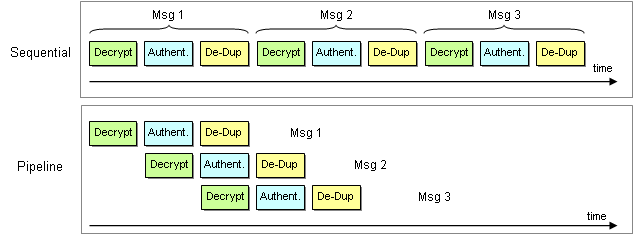
\includegraphics[width=0.8\textwidth]{kuvat/pipeline_processing.png}
      \caption{Kuva sanomien peräkkäisen käsittelyn ja prosessointiputken eroista \citep{Hohpe2004}\label{fig:pipelineprocess}}
      \end{center}
      \end{figure}

      Peräkkäisessä käsittelyssä, eli sanomat odottavat edellisen sanoman käsittely loppumista, sanomat joutuvat odottamaan toisten sanomien käsittelyä. Alemmassa prosessointiputkessa asynkronisuus mahdollistaa suodattimien operaatiot heti kun seuraava sanoma saapuu.
      
      Suodatinketjun suorituskykyä voidaan parantaa tästä entisestään. Edellisessä \ref{fig:pipelineprocess} prosessointiputken esimerkissä heikkoutena on se, että kaikesta hitain suodatinprosessi määrää koko järjestelmän sanomien käsittelytahdin. 
      Tässä tapauksessa hitain suodatin voidaan rinnakkaistaa. Haasteena on varmistaa, että jokaisen sanoman voi käsitellä vain yksi rinnakkaisista suodatinprosesseista. 
      Toinen huomioon otettava aspekti on, että rinnakkaistamminen ei takaa sanomien suoritusjärjestyksen säilymistä. Jos sanomien käsittelyjärjestyksellä on väliä, suodatinprosesseja voi olla vain yksi millä tahansa hetkellä. 
      Kolmas haaste on suodattimien tilanhallinta. Tilanhallinta rinnakkaisissa operaatioissa lisää tunnetusti kompleksisuutta, niin suodattimen tilanpalautuminen lähtöpisteeseen operaation valmistuttua yksinkertaistaa huomattavasti suodattimien rinnakkaistamista.

      Osittainen rinnakkaistaimisen  esimerkissä \ref{fig:parallelprocess} Hohpe ja Woof näyttävät miten salauksen purkamisen \textit{(decrypt)} käytetty suodatin voidaan rinnakkaistaa kolmeksi rinnakkaiseksi prosessiksi, koska purkamisoperaatio on työläin suodattimista \citep{Hohpe2004}.
      \begin{figure}[!h]
      \begin{center}
      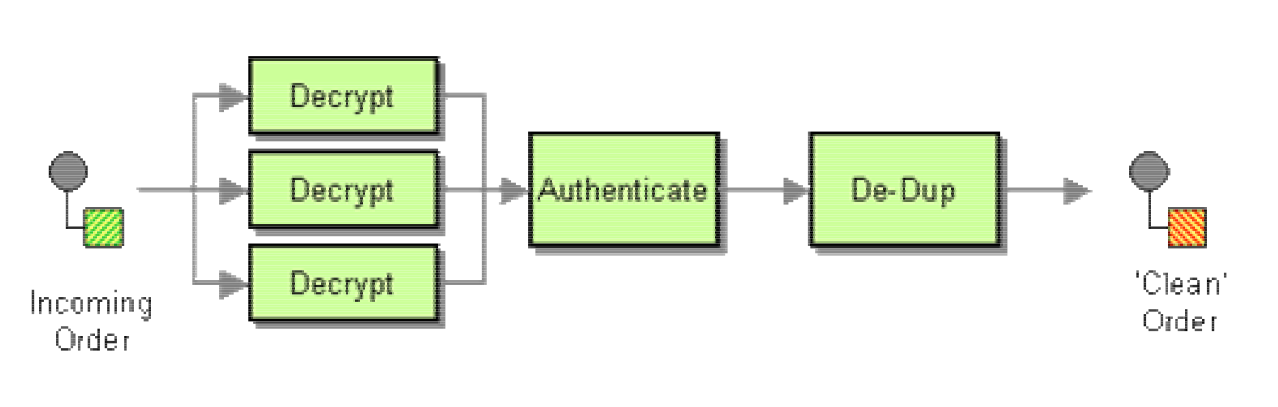
\includegraphics[width=0.8\textwidth]{kuvat/paraller_processing.png}
      \caption{Kuva sanomien rinnakkaisesta käsittelystä kun järjestyksellä on väliä \citep{Hohpe2004}\label{fig:parallelprocess}}
      \end{center}
      \end{figure}
      Esimerkissä duplikaattien tarkastus \textit{(de-dup)} on pidetty peräkkäisenä prosessina, koska duplikaattien havaitseminen tarvitsee sanomahistorian hyödyntämistä eli operaatio ei ole tilaton ja sen rinnakkaistaminen on haastavaa. 


   \textbf{Sanomareititin} \textit{(Message Router)}:
      Putkien ja suodattimien löyhät kytkennät mahdollistavat uuden prosessointiaskeleen lisäämisen olemassa olevien väliin. 
      Sanomareitittimen tapauksessa reititin vastaa putkien ja suodattamien suodatinta siinä suhteessa, että se tekee suorittaa prosessointia, mutta suodattimien sijaan reititin on kytketty useampaan ulostulo kanavaan. Reititin ei myöskään muokkaa sanomaa, vain on ainoastaan keskittynyt sanomien määränpään valitsemiseen.
      Reitittimen etuna on löyhä kytkentä muihin komponentteihin; ympärillä olevien suodattimien ei tarvitse olla tietoisia reitittimen olemassaolosta ja kaikki reitityspäätöksien logiikka elää yhdessä sijainnissa. Jos uusia sanomatyyppejä tai reititysmuutoksia toteutetaan, niin ainoastaan sanomareitittimen logiikka tarvitsee muokata. Koska saapuvan kanavan kaikki viestit siirtyvät reitittimen läpi yksitellen, on saapuvien viestien käsittelyjärjestys myös taattu.
      Löyhän kytkennän ylläpitohaasteet korostuvat sanomareititintä hyödyntäessä. Jos suurin osa järjestelmästä on löyhästi kytketty toiseen niin järjestelmän kokonaiskuvan muodostaminen käy hankalaksi. Hohpe ja Woofin mukaan näitä haasteita voi lieventää hyödyntämällä sanomien kulkuhistoriaa \citep[sivu~93]{Hohpe2004}.


      Reitittimen haasteina ovat erilaiset pullonkaulat. Reitittimestä voi syntyä ylläpidollinen pullonkaula, koska reitittimen pitää olla tietoinen kaikista vastaanottavista kanavista ja tästä voi syntyä ylläpidollinen ongelma varsinkin jos vastaanottokanavien lista vaihtuu tiheään. Toinen mahdollinen pullonkaula on suorituskyky. Reititin luonteensa vuoksi lisää ylimääräisen prosessointiaskeleen ja monissa sanomajärjestelmissä sanoman siirtäminen toiselle kanavalle vaati sanomien uudelleen koodausta. Useamman reitittimen rinnakkainen käyttö lieventää ongelmaa, mutta joka tapauksessa reititin tulee vaikuttamaan negatiivisesti sanomien viiveeseen vaikka sanomien käsittelytahti pysyisikin samana \citep[sivu~93]{Hohpe2004}.


      Reitittimen käyttö voidaan kategorioida useampaan eri tyyppiin. Yksinkertaisin reititin on kiinteä, jolloin sanoma kulkee yhdestä kanavasta yhteen vastaanottaja kanavaan. Kiinteiden reitittimen tarkoitus on irrottaa kiinteitä kytkentöjä erilaisista alijärjestelmistä tai välittää sanomia eri integraationratkaisujen välillä.
      Reititin voi olla sisältöpohjainen \textit{(content-based)} tai ympäristöpohjainen \textit{(context-based)}. Sisältöpohjainen tekee reitityspäätöksiä sanoman sisällön perusteella. Ympäristöpohjainen ottaa huomioon ympäristön tilan ja tekee esimerkiksi kuormituksen tasaamista tai uudelleenreititystä ympäröivän systeemin virhetilanteessa.
      Reitittimet voi jakaa tilallisiin ja tilattomiin; tilalliset reitittimet ottavat huomioon aikaisemmat sanomat ne voivat esimerkiksi estää duplikaattisanomien saapumisen tallentamalla jo saapuneet sanomat.
      Reitin voi olla myös dynaaminen \textit{dynamic router} ja vastaanottaa konfiguraatiomuutoksia ohjausväylän kautta. Tällä tavalla reititin voi muutta reitityslogiikkaansa ilman koodimuutoksia \citep[sivu~94]{Hohpe2004}.


   \textbf{Sanomankääntäjä} \textit{(Message Translator)}:
      Sanomankääntäjä on suodatintyyppi, joka mahdollistaa eri dataformaatteja käyttävät sovellukset keskustelemaan keskenään sanomien avulla. Hohpe ja Woof vertaavat sanomankääntäjä EIP:tä sanomajärjestelmille tarkoitetuksi versioksi tunnetusta sovitinsuunnittelumallista \citep[sivu~97]{Hohpe2004}, joka sai alkunsa Gang of Four teoksesta \citep{Gamma1994}.
      Kertauksena aikaisempiin esiteltyihin EIP: hin verrattuna sanomakääntäjän tarkoituksena on vähentää tiukkoja riippuvuuksia arkkitehtuurissa; sanomakanava mahdollisti, että sovellusten ei tarvitse tietää toistensa sijaintia, sanomareititin mahdollisti löyhät kytkennät sovellusten viestien reitittämisessä, joten sanomakääntäjä estää järjestelmien tiukat riippuvuudet toistensa dataformaateista.
      Sanomakääntäjä ratkaisee jaetun tietokannan haasteita jota käsiteltiin luvussa \ref{Tekniset lähestymistavat}. Erityisesti yhtenäisen skeemaan löytäminen ei muodostu ongelmaksi ja järjestelmät on  kytketty löyhemmin toisiinsa kääntäjiä hyödyntämällä.
      Vaihtoehtoinen lähestymistapa sanomakääntäjän sijaan olisi käyttää yhteistä datatyyppiä koko sanomajärjestelmässä, joka jakaa myös yhtäläisyyksiä jaetun tietokannan kanssa \ref{Tekniset lähestymistavat}, toteuttamalla sanoman datatyypin muunnokset sanomien päätepisteisiin \ref{Sanomien päätepiste}, mutta valmiissa kaupallisissa sanomajärjestlemiä tukevissa sovelluksissa päätepisteen koodi ei ole muokattavissa. Lisäksi sanomien kääntämislogiikan eläessä päätepisteessä, koodin uudelleenkäyttäminen on haastavaa.

      Hohpe ja Woof \citep{Hohpe2004} jakavat sanomakääntäjän operaatiot eri abstraktiotasoihin, ottaen löyhästi vaikutteita OSI-mallista \citep{OSImodel}, jakaen kääntämisoperaatiot kuljetus-, datan esitys-, datatyyppi- ja tietorakennekerroksiin (sovelluskerros).
      Kuljetuskerrokseen kuuluvat protokollat kuten http, mqtt, JMS. Datan esityskerros on kiinnostunut datan muodosta kuten JSON, XML ja enkoodauksesta kuten UTF-8. Datatyyppi viittaa soveluksen muistinsisäisiin esitystapoihin esim. ovatko postinumerot merkkijonoja vai kokonaisnumeroita ja ovatko esim. aikaleimat aina UTC-ajassa vai sisältävätkö aikavyöhykeinformaation.
      Tietorakennekerros (tai sovelluskerros) ottaa kantaa loogisiin kokonaisuuksiin, kuten eri dataentiteettien assosiaatioihin ja niiden kardinaliteetin esim. onko dataentiteettien välillä moni-moneen-yhteyksiä.
      Jakamalla kääntämisoperaatiot useampaan kerrokseen voidaan operaatioita käsitellä itsenäisesti omassa abstraktiotasossaan, kuten kuvassa \ref{fig:translationlayers}, ilman riippuvuutta muihin kääntäjiin ja kääntämisoperaation koodin uudelleenkäyttäminen on suoraviivaista. Myös eri abstraktiotasojen operaatiot ovat vaihdettavissa toisiin. Esimerkiksi datan esityskerroksessa \textit{(Data Representation)} voidaankin päättää, että data esitetäänkin JSON:ina CSV:een sijaan ilman, että vaihto aiheuttaa muutoksia muiden tasojen operaatioissa.

      \begin{figure}[h]
      \begin{center}
      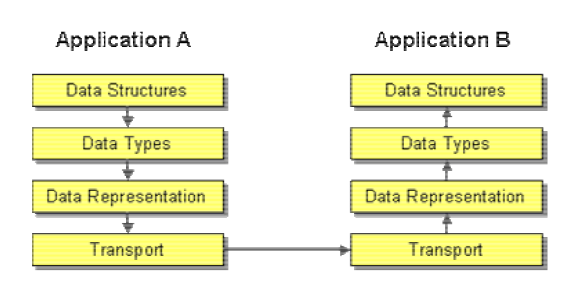
\includegraphics[width=0.8\textwidth]{./kuvat/translation_layers.png}
      \caption{Sanomakääntäjän operaatiot voivat kohdistua kaikkiin abstraktiotasoihin \citep{Hohpe2004}\label{fig:translationlayers}.}
      \end{center}
      \end{figure}

    \textbf{Sanomien päätepiste} \textit{(Message Endpoint)}\label{Sanomien päätepiste}:
      Verrattuna aikaisempiin esiteltyihin kattokategorian EIP:in, sanoman päätepiste on puuttuva palanen, joka mahdollistaa integroitavan sovelluksen liittämisen osaksi sanomaviestintää hyödyntävää kokonaisuutta; sanomien päätepiste on siis asiakasohjelmisto, joka yhdistää sovelluksen sanomakanavaan ja mahdollistaa sanomien lähettämisen tai vastaanottamisen. Sanomajärjestelmät ovat palvelinohjelmia ja sanomien päätepiste toimii niiden asiakasohjelmana. 
      Sanomien päätepiste vastaanottaa sovelluksen komennon tai datan ja muuttaa sen sanomaksi ja lähettää sanoman sanomakanavalle ja päinvastoin sanomia vastaanottavalle päätepisteelle. Hohpe ja Woof rajaavat yhden päätepisteinstanssin vain vastaanottamaan tai lähettämään, eikä toteuttamaan molempia eli sovellus hyödyntäisikin useampaa päätepistettä jos sen pitäisi kommunikoida useammalle sanomakanalle \citep[sivu~106]{Hohpe2004}. Sovellus voi kuitenkin hyödyntää useampaa päätepisteinstanssia vaikka sanomat lähtisivätkin vai yhdelle kanavalle, mahdollistaakseen instanssien skaalautumisen useammalle samanaikaiselle säikeelle.

      Päätepisteen koodi on räätälöity kyseiselle sovellukselle ja sanomajärjestelmän asiakasrajapinnalle sopivaksi. Päätepiste kapseloi sanomajärjestelmän sovellukselta joten sovellus ei ole tietoinen sanomajärjestelmästä. Esimerkiksi sanomajärjestelmän asiakasrajapinnan muutokset vaativat vain muutoksia päätepisteen koodiin ja integroitava sovellus on kapseloitu niin etteivät nämä muutokset vaikuta sen toimintaan.

      Päätepiste EIP:estä on muokattuja versioita riippuen siitä haluaako sanomia vastaanottava päätepiste käyttää erilaista vastaanottostrategiaa kuten kiertokyselyä tai tapahtumapohjaista reagointia. Useammat vastaanottavat päätepisteet voivat kilpailla sanomien käsittelystä \textit{(computing consumer)} tai jakaa viestin lähettämisen eri päätepisteelle sisäisen logiikan mukaan \textit{(message dispatcher)}. Vastaanottava päätepiste voi vastaavasti olla idempotenssi niin toistuivat sanomat eivät aiheuta järjestelmässä virhetiloja \citep[sivu~106]{Hohpe2004}.




      \chapter{Järjestelmäintegraatioiden suunnittelumallien kehitystä} \label{chap:kehitystä}

\section{Suunnittelumallien rooli nykypäivän ympäristössä}
   EIP-teoksen \citep{Hohpe2004} julkaisun jälkeen kirjailijat (pääasiassa Gregor Hohpe) ovat pyrkineet pitämään sisällön relevanttina. Vaikka kirjan arkkitehtuurisisältö itsessään on pysynyt relevanttina ja vaikuttaa selkeästi nykypäivän järjestelmäintegraatioratkaisuissa ja asynkronisten sanomien käytössä, on kirjan koodiesimerkit ja teknologiamaininnat vanhentuneet; näitä on myös tässä tutkielmassa pyritty korjaamaan tuoreemmilla esimerkeillä, jotka ovat tämän päivän opiskelijalle tuttuja. 


   Hohpen henkilökohtainen blogi sisältää useamman päivitetyn esimerkin tunnetuista EIP-suunnittelumallista, mutta nyt toteutettuna käyttäen pilviteknologioita: 
   \begin{itemize}
      \item Sisältöpohjainen reititin, EIP:een kategoriassa sanomien reititys, modernisoitiin käyttäen Googlen pilvialustan \textit{(GCP)} Google Cloud Functions palvelitonta arkkitehtuuria vuonna 2017 \citep{HohpeEIPGCP}. Alkuperäisen teoksen C\# Microsoft Message Queuing pohjainen toteutus vaihtui Node.js pohjaiseen, Google Cloud Pub/sub kirjastoa hyödyntävään toteutukseen.
   \item EIP-kirjassa esitelty monimutkaisempi esimerkki lainanvälittäjästä \textit{(Loan Broker)} \citep[sivu~317]{Hohpe2004} toteutettuun kolmella eri tavalla: Java / Apache Axis web-palvelimena, C\# / Microsoft Message Queuing sanomajonona ja Tibco ActiveEnterprise julkaise ja tilaa kanavana. Vuonna 2021 Hohpe aloitti sarjan blogikirjoituksia, joissa lainanvälittäjä esimerkki toteutetaan uudelleen käyttäen Amazon Web Services \textit{(AWS)} pilviteknologioita \citep{HohpeLoanAWS}.
      Lainanvälittäjä esimerkki toteutettiin pilvituotteilla AWS Step Functions, AWS Lambda, AWS Simple Notification Service, AWS Simple Queuing Service ja AWS DynamoDB. Katso kuva \ref{fig:hohpe_loanbroker_4}.

      \begin{figure}[h]
      \begin{center}
      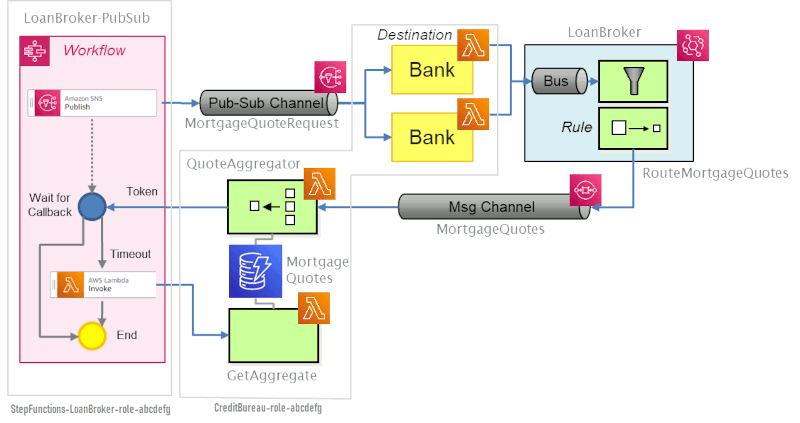
\includegraphics[width=0.8\textwidth]{kuvat/hohpe_loanbroker_4.png}
      \caption{Kuva EIP:een lainanvälittäjä esimerkistä AWS:än palveluita hyödyntämällä \citep{HohpeLoanAWS_4}\label{fig:hohpe_loanbroker_4}.}
      \end{center}
      \end{figure}


      Myöhemmissä sarjan osissa Hohpe keskittyy ohjelmiston julkaisemiseen AWS:ää hyödyntäen \citep{HohpeLoanAWS_4} \citep{HohpeLoanAWS_5}. Hohpe myös argumentoi, että EIP-suunnittelumallit ovat itse pilviarkkitehtuuriratkaisun lisäksi hyödyllisiä abstraktioita koodin julkaisua automatisoidessa \citep{HohpeLoanAWS_5}. Julkaisussa käytettävät teknologiat ovat AWS CloudFormation, AWS Simple Storage Service, AWS Serverless Application Model ja AWS Cloud Development Kit.

   \item Hohpen esimerkkien modernisointi jatkuu samana vuonna, lainanvälittäjä esimerkin siirtämisenä AWS:ltä Google Cloudille \citep{HohpeLoanGCP}.
      Ohjelman siirto ja kuvan \ref{fig:hohpe_loanbroker_4} AWS palvelut kuvaantuivat yksi yhteen GCP:een palveluille. Esimerkissä hyödynnettiin GCP Workflows, GCP Cloud Functions, GCP PubSub, GCP DataStore teknologoioita.
      Julkaisun automaatiossa huomattavaa oli, että AWS CloudFormationille ei löytynyt suoraa vastaavuutta GCP:een tarjonnasta ja vastaava toiminnallisuus pitää löytää kolmannen osapuolen ratkaisuista \citep{HohpeLoanGCP}.
   \end{itemize}

   EIP-teoksessa esiteltyjen suunnittelumallien esimerkkejä on myös vähitellen uudistettu EIP:een kotisivulle \citep{conversationPatterns}. Tällä hetkellä 67 suuniittelymallista 14 on modernisoitu. Modernisoidut on koottu yhteen paikkaan Hohpen blogiin \citep{HohpeModernExamples}. Aiemmin mainittujen pilvialustaesimerkkien lisäksi EIP-suunnittelumalleja on kyseisissä esimerkeissä toteutettu Golangilla, Apache Kafkalla, Apache Camelilla, Mule ESB:llä, RabbitMQ:lla ja Microsost Azurella.
   
   Edellä mainitut esimerkit, mukaan lukien listatut pilvialustaesimerkit, löytyvät julkisesta Githubissa isännöidystä tietovarastosta \citep{EIPModernGit}.


\section{Tilalliset protokollat}
EIP-suunnittelumallien heikkous on tilalliset \textit{(stateful)} protokollat. Tarve tilallisille protokollille on todettu 2017 integraatiotrendien analyysissä \citep{Ritter2017} 
Tämän lisäksi alkuperäisien EIP-kirjan kirjailijat ilmaisivat vuonna 2016, että tilallisien protokollien suunnittelumalleille on tarvetta, mikä voisi oikeuttaa toisen EIP-voluumin luomiseen \citep{Zimmermann2016}.
Hohpe on alkanut keräämään tilallisia suunnittelumalleja sivulle \citep{conversationPatterns}, mutta toistaiseksi suunnittelumallit eivät ole poikenneet uutta kirjaa. Verrattuna EIP-suunnittelumalleihin, Hohpen tilalliset mallit käyttävät sanomien sijaan keskusteluja \textit{(conversations)} jonka ympärille suunnittelumallien abstraktiot on rakennettu.


Integraatiotrendien ja kaupallisten sekä avoimen lähdekoodin alustojen  analyysissä todettiin, että lähes kaikki alustat tarjoavat omat tilalliset "keskustelunsa"~ja mahdollisuudet tallennustilan käyttöön \citep{Ritter2017}. Tosin tämä alustojen tarjoama tuki todetaan alkeelliseksi. Palvelukeskeisen arkkitehtuurin \textit{(Service Orieted Architecture, SOA)} kirjallisuudesta löytyy kuitenkin keskustelusuunnittelumalleja mitä ei löydy integraatioalustojen toteutuksista \citep{Ritter2017};
julkaisussa \citep{Barros2005} suunnittelumallit yhdestä-moneksi \textit{(one-from-many)} ja yhdestä-moneen \textit{(one-to-many)} ovat monenvälisiä keskustelusuunnittelumalleja jotka todetaan puuttuvan olemassa olevista toteutuksista \citep{Ritter2017}.

Koska nykypäivän integraatiot keskittyvät enemmän pilvipalveluhin, integraatiovaatimukset ovat alkaneet kallistua tilallisiin tallennustilaa vaativiin skenaarioihin mihin EIP ei vastaa ja kerätyt keskustelusuunnittelumallit ovat myös keskeneräisiä vastatakseen \citep{Ritter2017}. Paremmin muodostetuille keskustelusuunnittelumalleilla löytyisi tarvetta.

Huomioitavaa on, että keskustelusuunnittelumalleja ei voi kuitenkaan verrata palvelukeskeisen arkkitehtuurin koreografia- \textit{(choreography)} tai vuorovaikutussuunnittelumalleille \textit{(interaction patterns)}, koska 
keskustelumallit kuvaavat monimutkaisempia tehtäviä kuin datan lähettämisen ja vastaanottamisen \citep{Ritter2017}.

\section{Datavirtaprotokollat}
Synkronisia ja datavirtaprotokollia \textit{(streaming protocol)} ei ole huomioitu järjestelmäintegraatioissa eikä niiden suunnittelumalleissa, minkä Hohpe ja Woof myöntävät haastattelussa \citep{Zimmermann2016}. Erityisesti virtausprotokollien puute aiheuttaa haasteita esimerkiksi big data järjestelmien integraatioissa \citep{Ritter2017}.
Samassa haastattelussa Hohpe ja Woof toteavatkin, että virtausprotokollien suunnittelumallien dokumentointi parantaisi sanomien käytön ja virtauskäyttötapausten yhtäläisyyksien ymmärtämistä ja johtaisi EIP:een kaltaisten suunnittelumallien löytämiseen \citep{Ritter2017}.
Kirjailivat toteavat, että koko EAI ekosysteemistä puuttuu datavirtaprotokollien suunnittelumallit ja yhteiset protokollat \citep{Zimmermann2016}, mutta virtaprosessointia hyödynnettiin vuosi myöhemmin ainakin Jitterbitin ja Apache Camelin EAI-ratkaisuissa \citep{Ritter2017}.

Virtausdatan käsittelemistä EIP-malleilla on kokeiltu laitteistokiihdyttämisen kanssa hyödyntämällä ohjelmoitavia porttimatriiseja \citep{DannRitter2017}. Tutkimuksessa virtausdatan käsittelyä varten EIP-malleja laajennettiin kahdella uudella suunnittelumallilla: kuormituksen tasaaja \textit{(load balancer)} ja liittäjä reititin \textit{(join router)}. Kuormituksen tasaaja lähettää sanomaan yhteen useasta kanavasta hyödyntämällä yleisiä kuormituksen tasaus mekanismeja. Liittäjä reititin liittää useasta eri kanavasta saapuvat sanomat yhdelle kanavalle ohjelmoidun logiikan mukaisesti \citep{DannRitter2017}.


Akateeminen ja tekninen kirjallisuus integraatioista ja datavirroista jää vähälle vuoden 2017 jälkeen. Datavirtojen hallinnoinnista EAI-kontekstissa löytyy kuitenkin joku tuoreempi esimerkki \citep{WilkesPareek}, mutta kirja ei pyri suunnittelumallien kaltaiseen arkkitehtuuristandardisointiin. 
Tuoreita kaupallisten integraatioalustojen kirjoituksia datavirtojen hyödyntämisestä on julkaistu ja yksi suuri datavirtaus integraatioiden suosion ajaja näyttää olleen Apache Kafka \citep{WSO2Stream} \citep{IBMStream}; samanlaisia trendejä on myös nähtävissä dataintegraatioiden tutkimuspapereissa \citep{Bousdekis2021}.

\section{Virheenhallinta suunnittelumalleissa}
EIP-lähdeteos käsitteli niukasti virheenhallintaa. Teos sisälsi virheenhallinnan suunnittelumalleina kelvottomien sanomien kanavan \textit{(Invalid Message Channel)} johon sanomat, joiden käsittely päättyi virheeseen lähetetään, sekä toimittamattomien kirjeiden kanavan \textit{(Dead Letter Channel)} johon päätyneiden sanomien lähetys on epäonnistunut eikä sanoma pystynyt jatkamaan käsittelyään esimerkiksi järjestelmähäiriön takia \citep{Hohpe2004}.
Kirjailijat ovat myöhemmin avanneet virheenhallinnan sisällyttämisestä teokseen \citep{Hohpe2004} sillä, että virheenhallintastrategioiden käsittely vaatii kirjalta laajempaa sanastoa erityisesti tilanhallinnasta, mikä olisi paisuttanut teosta \citep{Zimmermann2016}.

Kaupallisissa ja avoimen lähdekoodin EAI-järjestelmissä virheenhallinta ja erityisesti poikkeuksien hallinnointi on kehittynyt pidemmälle kuin EIP-kirjallisuus \citep{Ritter2017}. Järjestelmät sisältävät yleensä systeemin kaikkien virheiden nappaamisen ja kaupalliset palvelut kuten Dell Boomi, IBM, SAP Cloud Integration ja Tibco sisältävät hienovaraisempia työkaluja virheiden vaikutusalan hallinnoimiseen \citep{Ritter2017}.

Tutkimukset \citep{ExceptionRitter2014} \citep{ExceptionRitter2016} ovat kartoittaneet EAI-järjestelmistä käytettyjä virheenhallintastrategioita ja pyrkineet mallintamaan niitä suunnittelumalleina. Virheenhallinnasta on siis tehty myös varsin kattavaa kartoitusta suunnittelumallien perspektiivistä.
Tapahtuman uudelleen yritys virheen tapahtuessa \textit{(retry pattern)} on yleinen suunnittelumalli joka ilmenee sanomakanavan tai yksittäisen tapahtuman tasolla ja yrittää operaatiota annetun määrän kertoja \citep{ExceptionRitter2014}.
Virheitä hallinnoidaan vikatilanne reitittimellä \textit{(failover router)} jossa sanoma reititetään vaihtoehtoisella kanavalle virheen tapahtuessa. Tämä suunnittelumalli eroaa alkuperäisen teoksen \citep{Hohpe2004} kiertotie EIP:stä \textit{(detour)} tarkastamalla jatkokäsittelyn EIP:tä kutsua ja reitittää vaihtoehtoiselle reitille ilman konfiguraatiosanomia.
Kompensointialue \textit{(compensation sphere)} on suunnittelumalli jossa prosessi tai aktiviteetti sisältää joukon korjaavia operaatioita (kompensointeja) jotka aktivoituvat eri virhetilanteista. Kompensoinnit voivat olla vain tiettyyn tilanteeseen reagoivia tai koko määriteltyyn alueeseen reagoivia \citep{ExceptionRitter2014}.

Tämän jälkeen EAI-järjestelmien virheenhallinta strategioita on tarkemmin lajiteltu erilaisiin suunnittelumalleihin \citep{ExceptionRitter2016}. Järjestelmien virheenhallintatavat kategorisointiin yhteentoista samankaltaiseen lähestymistapaan, jotka on esitetty taulukossa \ref{fig:exceptionritter}.


\begin{figure}[h]
\begin{center}
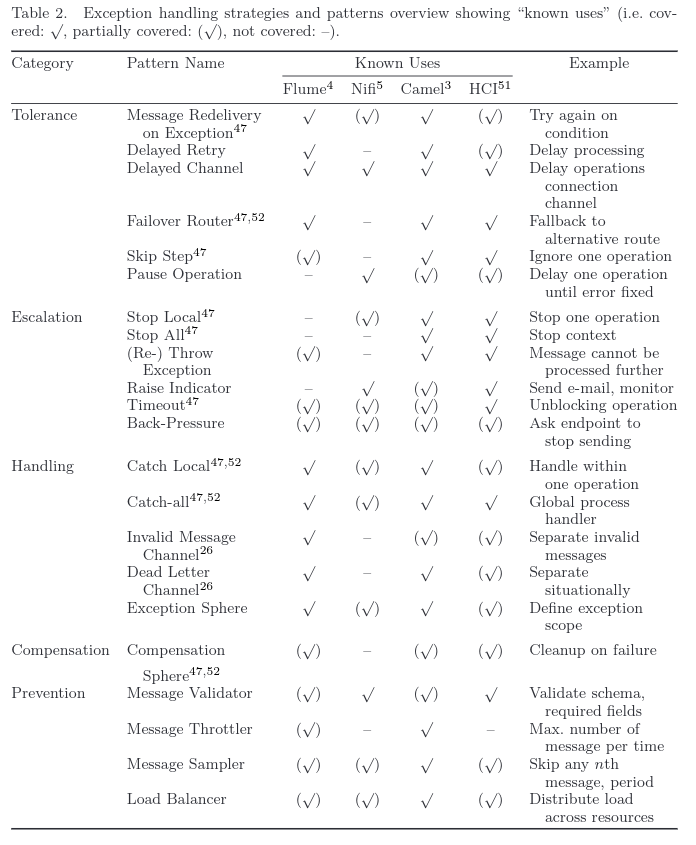
\includegraphics[width=0.8\textwidth]{kuvat/ritter_expetions.png}
\caption{Taulukko EAI-systeemien virheenhallinnan suunnittelumalleista ja niiden kategorioista \citep{ExceptionRitter2016}.\label{fig:exceptionritter}}
\end{center}
\end{figure}


Tutkimuksessa arvioitiin Apache Flume, Apache Cameli, Apache Nifi ja SAP HCI EAI-järjestelmien virheenhallintatapoja. Jos virheenhallintatapa esiintyi useammin kuin kerran, virheenhallintatapa sisällytettiin suunnittelumalliksi \citep{ExceptionRitter2016}.



\section{Suunnittelumallien formalisointi} \label{section:formalisointi}
EIP-suunnittelumallien formalisointi on kiinnostava aspekti erityisesti akateemisen kirjallisuuden kontekstissa. Formalisointi mahdollistaa suunnittelumallien matemaattisen analyysin ja varmentamisen ja takaisi varman pohjan järjestelmäintegraatioiden rakentamiselle suunnittelun ja ajon aikana.

Vuoden 2017 kartoitus \citep{Ritter2017} löysi yhden yrityksen formalisoida EIP:tä \citep{Fahland2013} jonka metodi formalisoinnille on hyödyntää värjättyjä Petri-verkkoja jossa värit kuvaavat datatyyppejä ja hallintasäikeet \textit{(control threads)} mallintavat kontrollirakenteita verkossa \citep{Fahland2013}.
Tämän jälkeen formalisointityötä on laajennettu vuonna 2021 \citep{Ritter2021}, jonka formalisointimetodi perustuu DB-verkoille \textit{(DB-nets)} \citep{Montali2017}; tutkimuksessa on pyritty rakentamaan vastuullinen formalisointitapa EIP-suunnittelumalleille, mikä täyttää EAI:in vaatimukset ohjausvuon, datan, ajan ja transaktioiden suhteen \citep{Ritter2021}. Jatkotutkimukseen tarpeen tutkimuksen tekijät löytävät EIP-yhdistelmien formalisoinnista, koska nykyinen tutkimus keskittyi yksittäisten EIP-suunnittelumallien formalisointiin \citep{Ritter2021}.

begin center latex
Formalisoinnin tutkimus on tuoretta ja keskenräistä verrattuna EIP-suunnittelumallien olemassaolon pituuteen. Suhteutettuna siihen kuinka paljon EIP:tä käytetään kaupallisissa ja avoimissa EAI-alustoissa, on nykyisen formalisoinnin keskeneräisyys harmillista, mutta viime vuosien uusiutunut kiinnostus aiheesta on lupaavaa. Ylipäätään EAI-teknologioiden formalisointi EIP-mallien ulkopuolella on keskittynyt palvelukeskeisen arkkitehtuurien ratkaisujen formalisointiin \citep{Ritter2017}.





\chapter{Yhteenveto}

EAI on terminä jo yli 20 vuotta vanha ja EAI-ratkaisut ovat vakiintuneet kiinteäksi osaksi ohjelmistoekosysteemiä. Tarve EAI-ratkaisuille kehittyi hajallaan olevista organisaatioiden järjestelmistä, jossa data saarekkeistui. Saarekkeet eivät keskustelleet toisilleen ja datan jakaminen eri järjestelmien välillä oli haastavaa.

Vaikka EAI-ratkaisuja löytyy monenlaisia, kaupallisia sekä avoimen lähdekoodin ratkaisuja, tästä huolimatta useimpien ratkaisujen lähestymistavat muistuttavat toisiaan.
Huomattava osa ratkaisuista muistuttavat toisiaan arkkitehtuurin ja suunnittelumallien osalta. Suuri osa näistä suunnittelumalleista perustuu sanomapohjaisiin lähestymistapoihin.
EAI-ratkaisuissa käytettyjen sanomapohjaisten suunnittelumallien perusta voidaan jäljittää 2004 julkaistuun EIP-kirjaan \citep{Hohpe2004}. Useimmat avoimen lähdekoodin liikepalveluväylät ovat omaksuneet kirjan mallikielen. 
EIP esittelee 67 sanomapohjaista suunnittelumallia, jotka on jaettu seitsemään eri kategoriaan.
EIP-suunnitelumallit sisältävät kuusi kattosuunnittelumallia joista muut suunnittelumallit johdetaan. Nämä kattosuunnittelumallit esittelevät tarvittavat konseptit, termit ja mallikielen, joista muut suunnittelumallit koostuvat. Nämä kattosuunnittelumallit ovat sanomakanava, sanoma, putket ja suodattimet, sanomareititin, sanomakääntäjä ja sanomien päätepiste.
Sanomapohjaisia suunnittelumalleja löytyy useiden EAI-ratkaisujen dokumentaatiosta, kuten myös pilvipalvelutarjoajien teknisistä blogeista. EIP-kirjalijat ovat myös pyrkineet modernisoimaan suunnittelumalleja nykypäivän pilviympäristöön ja hyödyntämään uusipia teknologiaratkaisuja.

Sanomapohjaisten suunnittelumallien tunnettu puute on tilallisuuden uupuminen. EIP-kirjan esittelemät mallit ovat lähes poikkeuksetta tilattomia. Tilallisten suunnittelumallien puute ei ole estänyt integraatioalustoja kehittämästä omia tilallisia lähestymistapojaan. Toinen tunnettu puute on datavirtaprotokollien huomioimattomuus, mikä aiheuttaa vaikeuksia big data-järjestelmissä. Lähteiden vähyys ei ole tässäkään tapauksessa estänyt kehitystä. Yksi datavirtojen hyödyntämisen ajajista on ollut Apache Kafkan suosio. Vastaavanlainen puute on myös virheenhallinta. EIP-kirja sisälsi vain kaksi virheenhallinta suunnittelumallia, mutta EAI-ratkaisut ovat kehittäneet omia mekanismejaan virheenhallitsemiseen ja tieteellinen kirjallisuus on pyrkinyt mallintamaan näitä lähestymistapoja ja muodostamaan niistä yleiskäytettäviä suunnittelumalleja.
Sanomapohjaisten suunnittelumallien kirjallisuutta on myös vaikeuttanut formalisoinnin puute, mikä on vaikeuttanut mallien syvempää analysointia. Analysointi on keskittynyt kahteen tapaan: värjättyihin Petri-verkkoihin ja ajoitettuihin DB-verkkohin. Jälkimmäisen metodin pyrkiessä ottamaan enemmän huomioon sanomapohjaisten suunnittelumallien elementtejä. Kirjallisuus formalisoinnille on myös kohtuu tuoretta.

Sanomapohjaiset suunnittelumallit ovat olleet vaikutusvaltainen aspekti EAI-ratkaisujen kehityksessä, mikä näkyy myös nykypäivän pilviratkaisujen lähestymistavoissa. Isoa osaa alkuperäisten EIP-suunnittelumallien puutteista on paikattu niiden implementaatioissa ja myöhemmässä kirjallisuudessa; formalisoinnin puutteellisuuden vaikuttaessa negatiivisesti suunnittelumallien tieteelliseen kirjallisuuteen.


Taulukoihin \ref{table:eip1} ja \ref{table:eip2} on tiivistetty tutkielman lopputuloksia. Taulukot sisältävät viisi parhaiten tuettua EIP-suunnittelumallia. Järjestyksenä ensimmäisenä ovat suunnittelumallit, joille löytyy parhaiten edes osittainen tuki eri integraatioalustoilta, perustuen tutkimukseen \citep{Ritter2017}.
Kaikki listatut suunnittelumallit ovat alkuperäisen EIP-kirjan \citep{Hohpe2004} suunnittelumalleja ja kaikki listatut mallit ovat myös tilattomia.
Modernisoitu on rajattu EIP-suunnittelumallien omiin modernisointi toimiin \citep{HohpeModernExamples}. Formalisoinnissa on keskitytty luvussa \ref{section:formalisointi} käsiteltyihin metodeihin eli värjättyihin Petri-verkkoihin ja DB-verkkoihin.

\begin{table}[h]
\centering
    \begin{tabular}{|p{0.19\textwidth}|p{0.25\textwidth}|p{0.2\textwidth}|p{0.2\textwidth}|}
    \hline
    Suunnittelumalli & Tuki & Modernisoitu & Formalisointi \\ \hline
    Jakaja \textit{(Splitter)} &
        \begin{itemize}
            \item 12/15 alustassa täysi tuki \citep{Ritter2017}.
            \item 1/15 alustassa osittainen tuki \citep{Ritter2017}.
        \end{itemize}
      &
        \begin{itemize}
            \item Ei
        \end{itemize}
      &
        \begin{itemize}
           \item DB-verkko formalisointi esimerkki \citep{Ritter2021}.
        \end{itemize}
    \\ \hline
    Sanomakääntäjä \textit{(Message Translator)} & 
        \begin{itemize}
            \item 8/15 alustassa täysi tuki \citep{Ritter2017}.
            \item 5/15 alustassa osittainen tuki \citep{Ritter2017}.
        \end{itemize}
      &
        \begin{itemize}
            \item Ei
        \end{itemize}
      &  
        \begin{itemize}
           \item DB-verkko formalisointi esimerkki \citep{Ritter2021}.
           \item Värjätty Petri-verkko formalisointi esimerkki \citep{Fahland2013}.
        \end{itemize}
      \\ \hline
    Sisältöpohjainen reititin \textit{(Content Based Router)} & 
        \begin{itemize}
            \item 11/15 alustassa täysi tuki \citep{Ritter2017}.
            \item 1/15 alustassa osittainen tuki \citep{Ritter2017}.
        \end{itemize}
      &
        \begin{itemize}
           \item Kyllä. Modernisoitu esimerkki Apache Camelille \citep{HohpeModernExamples}.
        \end{itemize}
      &
        \begin{itemize}
           \item DB-verkko formalisointi esimerkki \citep{Ritter2021}.
        \end{itemize}
      \\ \hline
    \end{tabular}
   \caption{Taulukko yleisimpien EIP-suunnittelumallien ominaisuuksista.}
   \label{table:eip1}
\end{table}



\begin{table}[h]
\centering
    \begin{tabular}{|p{0.19\textwidth}|p{0.25\textwidth}|p{0.2\textwidth}|p{0.2\textwidth}|}
    \hline
    Suunnittelumalli & Tuki & Modernisoitu & Formalisointi \\ \hline
    Sisällön rikastaja \textit{(Content Enricher)} & 
        \begin{itemize}
            \item 6/15 alustassa täysi tuki \citep{Ritter2017}.
            \item 6/15 alustassa osittainen tuki \citep{Ritter2017}.
        \end{itemize}
      &
        \begin{itemize}
           \item Kyllä. Modernisoitu esimerkki käyttäen Amazon EventBridge Pipes pilvipalvelua \citep{HohpeModernExamples}.
        \end{itemize}
      &
        \begin{itemize}
           \item DB-verkko formalisointi esimerkki \citep{Ritter2021}.
           \item Värjätty Petri-verkko formalisointi esimerkki \citep{Fahland2013}.
        \end{itemize}
      \\ \hline
    Sisältösuodatin \textit{(Content Filter)} & 
        \begin{itemize}
            \item 5/15 alustassa täysi tuki \citep{Ritter2017}.
            \item 7/15 alustassa osittainen tuki \citep{Ritter2017}.
        \end{itemize}
      &
        \begin{itemize}
            \item Ei
        \end{itemize}
      &
        \begin{itemize}
           \item Ei formalisointiesimerkkejä \citep{Ritter2021}.
        \end{itemize}
      \\ \hline
    \end{tabular}
   \caption{Taulukko yleisimpien EIP-suunnittelumallien ominaisuuksista.}
   \label{table:eip2}
\end{table}



\chapter*{Tekoälyn käyttö tutkielmassa}
Tutkielman käytössä hyödynnettiin kielimalleja ChatGPT ja Microsoft CoPilot. Kielimalleja hyödynnettiin tutkielman jaottelun ideoitiin ja lähteiden etsimiseen. Kumpikaan käyttökohde ei vaikuttanut tutkielman lopputulokseen kielimallien liian hallunisoinnin vuoksi.

